\documentclass[11pt]{article}
\usepackage{royden-report}
\usepackage[T1]{fontenc}
\usepackage{lmodern,microtype,array,longtable,enumitem}
\setlist{itemsep=3pt,topsep=5pt}
\newcommand{\absD}{\lvert D_\tau\rvert}
\newcommand{\model}{\texttt{water-\allowbreak wave-\allowbreak dysthe-\allowbreak spatial-v1}}
\DeclareMathOperator{\sech}{sech}
\DeclareMathOperator{\Repart}{Re}
\title{Dysthe Solitary Waves and the Published Tests}
\author{Literature review and computational audit}
\date{27 October 2026; revised after the cluster-results push}
\begin{document}
\maketitle
\begin{abstract}
The defensible research target is to determine which resolved water-wave
Dysthe solitary profiles remain close to their symmetry orbits over a measured
propagation interval, and whether neural approximations reproduce that behavior.
Two September 2026 preprints refine the theoretical context, but neither supplies
an orbital-stability theorem for the implemented periodic free-surface model.
The newly pushed cluster snapshot reports qualified periodic references through
$\xi=64$, but none of 24 evaluated neural fits passes the combined $\xi=4$ gates;
12 random-field fits have execution errors. Detailed reference and failure
records remain unpublished. A fresh projection audit shows that copying the generic-packet neural
cutoff to the solitary-wave domain would impose a 66.1\% relative $H^2$ error
before optimization. This report distinguishes literature results, published
measurements, local historical evidence and proposed tests.
\end{abstract}

\section{The question and the exact equation}
The project's original question is whether solutions remain smooth over
increasing propagation distance. Solitary waves provide a controlled family
with which to investigate this question, but existence of one traveling profile
does not establish global existence for arbitrary initial data.

The active model evolves a scaled complex \emph{free-surface envelope}
$u(\xi,\tau)$ in downstream distance $\xi$, with retarded-time coordinate $\tau$:
\begin{equation}\label{eq:dysthe}
\begin{aligned}
u_\xi=F(u)={}&-iu_{\tau\tau}-i|u|^2u\\
&-\epsilon\bigl(8|u|^2u_\tau+2u^2\overline{u_\tau}
               +2iu\absD(|u|^2)\bigr).
\end{aligned}
\end{equation}
This is the spatial Fedele--Dutykh free-surface convention \cite{fd}.
Its model identifier is \model. The Fourier multiplier of $\absD$ is $|k|$ and that of
$\partial_\tau$ is $ik$; thus $\mathcal H\partial_\tau=\absD$.
The potential-envelope equation, a temporal equation, and a two-dimensional
model are different contracts. Their results cannot be imported by name alone.

\begin{definition}
A traveling solitary envelope on the line has the form
\begin{equation}\label{eq:travel}
u(\xi,\tau)=e^{-i\mu\xi}Q(\tau-s\xi),\qquad Q(z)\longrightarrow0
\quad\text{as }|z|\longrightarrow\infty.
\end{equation}
The profile satisfies $F(Q)+i\mu Q+sQ'=0$. A large periodic box approximates
this setting only after a separate domain-sensitivity check.
\end{definition}

At $\epsilon=0$ and $s=0$, the focusing NLS seed is
$Q_0(z)=\sqrt{2\mu}\sech(\sqrt\mu z)$, $\mu>0$. At nonzero $\epsilon$ it is
generally only an initial guess. Both the complex phase and shape must satisfy
the full Dysthe profile equation. The solitary object is an envelope of many
carrier crests, rather than one permanently isolated surface crest.

\newpage
\section{What the current literature establishes}
\paragraph{Direct numerical precedent.}
Fedele and Dutykh constructed spatial Dysthe traveling waves with a
Petviashvili iteration and studied their collisions numerically
\cite{fd}. Their observed inelastic interactions are an established benchmark,
not a new discovery to claim from this project. Convergence of that profile
iteration is not dynamical stability. Earlier perturbative work by Akylas
described how higher-order modulation changes an initially NLS-like solitary
envelope, including amplitude and speed adjustments in the studied regime
\cite{akylas}. This motivates comparing an exact NLS inlet with a corrected
Dysthe profile.

\paragraph{A 2026 existence result, with a coefficient restriction.}
Esfahani, Kairzhan and Karazym's preprint, revised 21 September 2026, proves
parameter-dependent traveling-wave existence and nonexistence for a general
nonlocal derivative NLS family \cite{ekk}. In their convention,
\[
iu_t-u_{xx}-b|u|^2u+i\alpha|u|^2u_x+i\beta u^2\bar u_x
 +\gamma u\partial_x\mathcal H(|u|^2)=0.
\]
Matching \eqref{eq:dysthe} gives
\[
(b,\alpha,\beta,\gamma)=(1,8\epsilon,2\epsilon,-2\epsilon).
\]
Their main existence theorems assume $\gamma\geq0$; their other negative-$\gamma$
existence regime requires a vanishing reduced quintic coefficient, whereas ours
is $B=-35\epsilon^2/4$. Hence those results do not directly prove existence for
this branch. They also explicitly leave stability and instability unaddressed.
This is a useful analytical framework, not a certificate for the current solver.

\paragraph{A sharper 2026 obstruction to NLS-type integrability.}
Sutherland and Yim's 19 September 2026 preprint computes resonant six-wave
scattering in Hamiltonian Dysthe models \cite{sy}. Its spatial free-surface
case is connected to our coefficients by the Fedele--Dutykh gauge transformation,
including the induced quintic term. Under its stated formal-functional and
regularity assumptions, the result excludes an infinite conserved hierarchy
with independent regular $C^3$ quadratic leading symbols beyond
$\operatorname{span}\{1,k,k^2\}$. It does not exclude every conceivable notion of
integrability, solitary profiles, or stable propagation. The analysis uses
continuous Fourier variables on the line; it is not a periodic-box stability
theorem. Both 2026 papers are preprints, not verified journal publications in
the records inspected.

\paragraph{Coherent events are broader than exact solitary waves.}
Schober and Islas's 2025 study uses Floquet spectra to examine soliton-like rogue
events in conservative and dissipative higher-order NLS settings \cite{si2025}.
Its publisher abstract was accessible; its full text was not inspected here.
Tikan et al. connect random narrowband water-wave fields, coherent-pulse signatures
and nonlinear dispersion measurements with NLS/Dysthe/Euler comparisons
\cite{tikan}. These support later random-input diagnostics, not a claim that
every large peak is a soliton. The supplied 2026 Schober--Islas preprint concerns
weak viscosity and mean-flow damping \cite{si2026}; such terms require a
separately versioned extension, and are not part of \eqref{eq:dysthe}.

\newpage
\section{Four claims that must remain separate}
\begin{enumerate}
\item \textbf{Profile existence:} a nontrivial $Q$ solves the traveling-wave
equation. A small computed residual is numerical evidence; an existence theorem
needs an analytical or validated numerical argument.
\item \textbf{Spectral stability:} the correct linearized evolution has no
growing modes in a specified function space. A finite matrix calculation must
be checked against resolution and domain changes.
\item \textbf{Finite-distance robustness:} selected small perturbations stay
close to the traveling-wave orbit over the tested interval. This can be measured
with resolved simulations.
\item \textbf{Global orbital stability or global regularity:} a uniform statement
for all sufficiently small perturbations, or continuation for general data at
arbitrary distance. The present tests do not establish either statement.
\end{enumerate}

The phrase \emph{soliton} is used variably in this literature. Here, ``solitary
wave'' describes a persistent localized traveling profile; ``integrable soliton''
additionally invokes the special scattering structure of an integrable model.
Nonintegrability does not imply that every solitary wave is unstable. Likewise,
a transient focusing event or a breather need not be a traveling profile.

The small-data global well-posedness and scattering theorem of Mosincat, Pilod
and Saut concerns a Dysthe equation on $\RR^2$ \cite{mps}. Its dimensional and
evolution setting differs from this one-coordinate periodic spatial solver.
It cannot be presented as a theorem covering our solitary profiles or arbitrary
large-amplitude data. No directly applicable orbital-stability theorem for the
exact implemented model was found in the sources reviewed; this is a literature
search conclusion, not a proof that no such result exists.

\subsection{What ``long term'' means operationally}
There is no universal terminal value of $\xi$, amplitude or $H^2$ norm that
establishes long-term stability. Record the actual interval together with
natural propagation scales. With $A_0=\|u(0)\|_\infty$, the current campaign uses
\[
N_{\rm nl}(\Xi)=A_0^2\Xi
\]
as an initial-peak nonlinear-distance convention. For a traveling wave also
record $|\mu|\Xi/(2\pi)$ phase cycles and the shift $s\Xi$ relative to its width.
For the stored solitary profile, $A_0=1.958116$: the completed $\Xi=0.1$ check
covers $0.3834$ nonlinear lengths, whereas the proposed $\Xi=20$ study would
cover $76.68$. This is a meaningful increase in scope, not an existing result.

In the model normalization, $\xi=\epsilon^2k_0X$ and
$\tau=\epsilon(2k_0X-\omega_0T)$. Thus physical distance is
$X=\xi/(\epsilon^2k_0)$ once the carrier is specified. The approximation need
not remain physically accurate at arbitrarily large $X$, even if its numerical
solution stays smooth. Track effective steepness and spectral bandwidth; use
water-wave experiments or higher-fidelity water-wave models for physical validation.

\newpage
\section{Audit of the pushed tests and recorded results}
The inspected remote workstream is
\href{https://github.com/matasvai/dysthe-experiments/tree/codex/long-distance-a100}{\texttt{codex/long-distance-a100}},
at commit
\begin{center}\small\texttt{723883f27a6b3489bfc36f55d9d15b52e8635ad0}.\end{center}
This new push adds 29 result files to the previously reviewed code commit
\texttt{c04b44ba}. It includes a \texttt{gpu2} cluster snapshot as well as the
earlier CPU results. The 39-test software check remains applicable to the
unchanged source; it is distinct from the scientific accuracy gates. The new
snapshot and its limits are examined below. The earlier report's statement
that no cluster results were published is superseded by this revision.

\subsection{The CPU pilot supports slabs, with limited scope}
The completed pilot used 18 initial fields: six each of packets, modulated
backgrounds and smooth random Fourier fields. Twelve trained the operators;
three validated and three tested them. PINNs were fitted separately per inlet.
Two optimization seeds give six test case--seed pairs, but only three independent
test fields. All methods used a small budget; FNO rollout and a per-inlet PINN
solve have different inference tasks and must not be treated as identical services.

\begin{table}[h]\centering\small
\begin{tabular}{lrrrr}\toprule
Method & $L^2$ (\%) & $H^1$ (\%) & Peak (\%) & Pairs passing\\\midrule
Global PINN & 1.995 & 3.041 & 0.936 & 2/6\\
NLS-warm PINN & 2.074 & 3.560 & 1.285 & 3/6\\
Four-slab PINN & 0.963 & 1.881 & 1.089 & 6/6\\
FNO & 58.739 & 58.843 & 32.698 & 0/6\\
PINO & 56.617 & 56.833 & 34.592 & 0/6\\\bottomrule
\end{tabular}
\caption{Published CPU measurements: worst saved-station relative errors through
$\xi=2$. Gates were 1\% complex $L^2$, 5\% $H^1$ and 5\% peak error.
No phase or translation alignment was applied. Source: archived
\texttt{data/cpu-errors.csv}.}
\end{table}

\begin{figure}[h]\centering
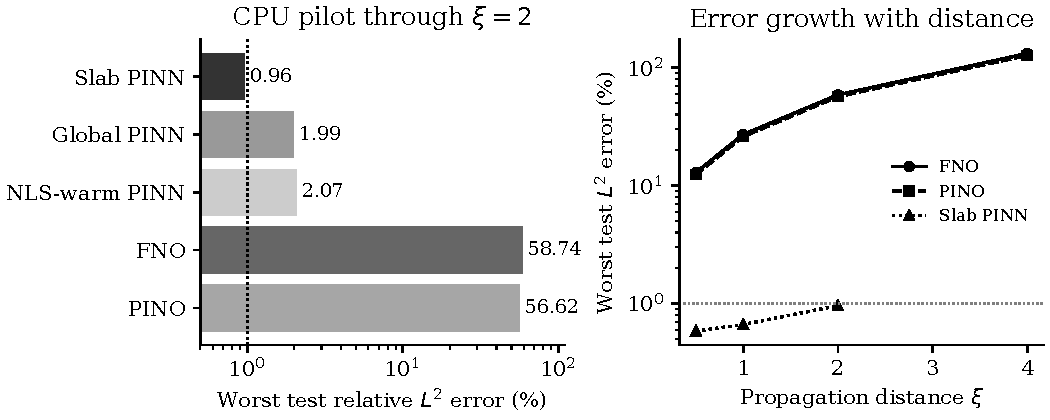
\includegraphics[width=\textwidth]{figures/cpu-comparison.pdf}
\caption{Replot of recorded CPU results. The slab PINN was fitted over each
interval; the operators were rolled out beyond their short training windows.
These are neither solitary-wave tests nor A100 measurements.}
\end{figure}

\newpage
\subsection{What the existing results imply for method selection}
The slab PINN is the most promising \emph{tested neural method} for the current
per-inlet task. It is not yet the fastest solver. Recorded median fitting time
was about 1.26 seconds per inlet, versus about 0.0294 seconds for a coarse
numerical solve through $\xi=2$. The latter had worst test $H^1$ error about
$4.62\times10^{-7}$. These preliminary CPU timings were not an isolated,
matched-accuracy benchmark; some training overlapped and setup/audit costs were
excluded. They do not establish neural speedup.

The trained FNO and PINO are not reliable long-distance predictors: neither
passed all test gates even through $\xi=0.5$. Their $\xi=4$ errors exceeded
100\%. Twelve operator-training inlets and a small budget are insufficient to
draw a general conclusion about FNO, but these particular checkpoints should
not be promoted as a solver. NLS warm-starting also failed to improve the
aggregate PINN result under this budget.

Three numerical validation fields were independently refined through $\xi=16$;
recorded sampled $H^2$ norms remained finite, with maximum approximately 4.224.
These are finite-distance periodic observations. The new cluster snapshot
extends the recorded numerical coverage below; neither set establishes
solitary-wave stability or continuum existence.

\subsection{The pushed long-distance campaign is a sound staged design}
\begin{center}\small
\begin{tabular}{p{.18\textwidth}p{.17\textwidth}p{.56\textwidth}}\toprule
Stage & Distances $\xi$ & Purpose and required observation\\\midrule
Reference & 4, 8, 16, 32, 64 & Independently refine grid and step; track $H^2$,
spectral tails, action and the NLS control. Stop an unresolved inlet.\\
Slab PINN & 4, 8, 16 & Require saved-station complex $L^2\leq1\%$, $H^1,H^2\leq5\%$
and peak error $\leq5\%$. Stop later fits after failure.\\
Sensitivity & 4, 8, 16 & Check signed response with perturbation halving and
independent reference refinements; 1\% response agreement.\\
Packet domain & 4, 8, 16, 32, 64 & Compare the same analytic localized inlet on
two periods; require initial agreement and 1\% $H^1$ domain agreement.\\\bottomrule
\end{tabular}
\end{center}
The production design has six validation and six test inlets across three
families, with neural seeds 11, 29 and 47. Each PINN is fitted anew; the
4/8/16 horizon fits retrain early slabs independently. Training-reserved inputs
are not used to train an FNO in this campaign. A100 access therefore scales the
selected per-inlet experiment; it does not already implement operator generalization.

The published tiny workflow completed 24 case/stage tasks. One PINN failed its
accuracy gate at $\xi=0.2$, both packet-domain tests failed their coarse-domain
criteria, and four domain tests were correctly marked inapplicable. All six
reference and sensitivity checks completed. These retained failures are useful:
workflow completion is not ``all scientific gates passed.'' Replaying completed
fits preserved 180 artifact hashes; this is CPU reuse evidence, not CUDA restart
equivalence. Allocation-specific CUDA checks remain essential.

\newpage
\subsection{Newly published cluster results: the actual outcomes}\label{sec:gpu}
The new \texttt{results/long-distance-gpu2-2026-10-26} snapshot changes the
evidence status. Its configuration matches the production design. Its manifest
identifies source commit \texttt{c04b44ba}; all eight recorded source hashes
match the previously tested pinned sources. All 28 published metadata files
match their manifest hashes and byte lengths; the manifest is the 29th file.

\begin{center}\small
\begin{tabular}{p{.23\textwidth}p{.68\textwidth}}\toprule
Stage & Recorded result in the new summary\\\midrule
Periodic reference & 12/12 qualified through $\xi=64$.\\
Numerical sensitivity & 12/12 qualified through $\xi=16$.\\
Packet domain & Four pass $\xi=4$, fail $\xi=8$; eight nonpackets inapplicable.\\
PINN accuracy & 0/24 evaluated packet/sideband fits qualify through $\xi=4$.\\
PINN execution & 12 random-field fits: execution errors, no accuracy results.\\
Later PINN horizons & No evaluated $\xi=8$ or $16$ results; campaign incomplete.\\\bottomrule
\end{tabular}
\end{center}

Each validation/test split has 12 of 18 requested case--seed pairs evaluated,
representing four of six independent inlets. Both evaluated families are
represented, but the random family is absent. The following are therefore
\emph{incomplete-subset} statistics; failed executions cannot be counted as
accurate predictions or omitted from the coverage statement.

\begin{table}[h]\centering\small
\begin{tabular}{lrrrr}\toprule
Split/statistic & $L^2$ (\%) & $H^1$ (\%) & $H^2$ (\%) & Peak (\%)\\\midrule
Validation worst & 1.968 & 5.826 & 30.741 & 1.383\\
Validation median & 1.347 & 3.419 & 14.681 & 0.820\\
Test worst & 1.577 & 4.130 & 22.115 & 1.498\\
Test median & 0.934 & 2.968 & 14.900 & 0.669\\
Acceptance gate & 1.000 & 5.000 & 5.000 & 5.000\\\bottomrule
\end{tabular}
\caption{Recorded interval errors through $\xi=4$. Medians are across the
12 evaluated case--seed maxima in each split, not across all requested inputs.
Detailed $H^2$ traces were not included in the pushed snapshot.}
\end{table}

\begin{figure}[h]\centering
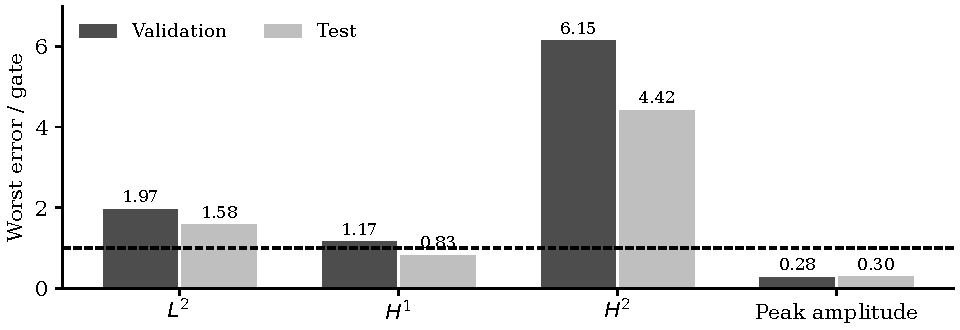
\includegraphics[width=.93\textwidth]{figures/gpu-gates.pdf}
\caption{Worst reported errors divided by their acceptance thresholds.
A value above one fails that metric. The derivative-sensitive $H^2$ error is
the largest violation; no successful long-distance neural result is established.}
\end{figure}

\newpage
\subsection{What the new results mean for the research goal}
\paragraph{Derivative accuracy is the decisive new issue.}
Eleven of the 24 evaluated fits pass the earlier CPU pilot's $L^2$, $H^1$ and
peak criteria, including all six evaluated test-sideband fits. Their individual
\texttt{sampled\_interval\_pass} flags are true because that older flag excludes
$H^2$. All 24 fail the long-distance gate that includes $H^2$; for those eleven,
the extra derivative criterion causes rejection. Use the full campaign status,
not the older flag, when reporting success. Initial gate violations occur between
$\xi=0.30$ and $1.10$, although each evaluated fit was trained through 4.

This is directly relevant to the smoothness objective: a good envelope or peak
prediction can conceal inaccurate derivatives. An $H^2$ error of 22.1\% is an
\emph{approximation error relative to the reference}, not a 22.1\% growth in
the true norm and not evidence of a singularity. Its cause cannot be inferred
from aggregate errors alone. Inspect per-mode error and residuals to distinguish
spurious high-frequency content, truncation, phase drift and optimization error.
The earlier CPU result and this run differ in inlets, horizon, network, bandwidth,
budget and acceptance criteria; the change cannot be attributed to GPU execution.

\paragraph{Periodic qualification and isolated packets have different limits.}
The summary records reference qualification through 64, but all packet domain
checks fail at 8. Thus the recorded periodic numerical evidence extends much
farther than the declared doubled-domain agreement test, which passes only
through 4. This is not a whole-line certificate. The detailed records are needed
to distinguish finite-box interaction from failed refinement. Likewise, sensitivity
qualification through 16 is not a bound on the size of amplification: it says
the prescribed response comparisons passed. The actual norms, amplification
curves and qualification margins are not in the uploaded summary.

\paragraph{Execution and provenance limits.}
All 24 completed PINN records include positive GPU allocations, with reported
peak allocated tensor memory 94,955,520 bytes (90.56 MiB). Their median recorded
optimization time is 62.61 seconds (range 47.63--67.44). This is not total device
memory or a matched CPU/GPU speed comparison. CUDA 12.8 and PyTorch
\texttt{2.10.0+cu128} are recorded. The exact GPU model, node and scheduler
allocation are not in the published records; the declared \texttt{gpu2}
campaign targets A100 hardware. Job and runtime-lock files are only hash-listed.
The random-fit exception logs are absent, so neither memory exhaustion nor an
optimizer failure can be asserted as their cause.

\paragraph{Next decision.}
Retrieve the detailed numerical \texttt{result.json} files, the PINN $H^2$
traces and \texttt{tasks/pinn-024.json} through \texttt{pinn-035.json} before
diagnosing the missing random fits. Use validation cases to test shorter slabs,
resolved bandwidth and optimization settings under controlled budgets. Do not
automatically extend failed fits to larger distances. Freeze any selected repair
before evaluation on a new untouched test set. These generic-wave results inform
the learning method; they still do not test solitary-wave stability.

\newpage
\section{The solitary-wave implementation and a new resolution audit}\label{sec:projection}
The local solitary-wave code computes a conjugate-reflection-symmetric profile,
then propagates it without enforcing that symmetry. A historical smoke at
$\epsilon=0.025$, $\mu=2$, $s=0$, $L=160$, $N=4096$ reached only $\xi=0.1$.
Its full profile residual was $2.03\times10^{-11}$ and unperturbed final relative
complex $L^2$ error was $7.09\times10^{-11}$. Its field checksum was verified
against the stored report. This checks consistency over a short interval.

The standalone solitary files and their refinement configuration are local,
untracked work, absent from the audited pushed tree. Their loader still depends
on a historical profile file/sidecar even in recompute mode. The long-distance
cluster campaign uses generic inlets, not solved solitary profiles. No completed
refined long-distance solitary study, real-linear stability spectrum, or
solitary-specific PINN/FNO result was found.

\subsection{Fourier representation can defeat the test before training}
On a periodic grid of length $L$, let $k_m=2\pi m/L$ and
$\widehat Q_m=\operatorname{FFT}(Q)_m/N$. Define
\begin{equation}\label{eq:floor}
p_r(K)^2=\frac{\sum_{|m|>K}(1+k_m^2)^r|\widehat Q_m|^2}
                 {\sum_m(1+k_m^2)^r|\widehat Q_m|^2}.
\end{equation}
Since Fourier modes are orthogonal in these discrete $H^r$ norms, every
approximation supported in $|m|\leq K$ has relative error at least $p_r(K)$.
This statement follows by splitting its squared error into retained and
discarded Fourier modes. Phase and translation alignment preserve the support
and cannot eliminate this floor.

\begin{table}[h]\centering\small
\begin{tabular}{rrrrr}\toprule
$K$ & $k_{\max}$ & $p_0$ (\%) & $p_1$ (\%) & $p_2$ (\%)\\\midrule
48 & 1.885 & 19.146 & 38.520 & 66.086\\
96 & 3.770 & 2.989 & 10.074 & 27.467\\
192 & 7.540 & 0.08096 & 0.50049 & 2.44868\\
256 & 10.053 & 0.007532 & 0.060796 & 0.386883\\
384 & 15.080 & 0.0000664 & 0.0007879 & 0.0073469\\\bottomrule
\end{tabular}
\caption{New calculation on the stored $L=160$ Dysthe profile; not a new
propagation or neural-training experiment. The same-grid NLS seed also has a
59.77\% $H^2$ floor at $K=48$. Data and source hashes accompany the report.}
\end{table}

The published neural cutoff $K=48$ belongs to $L=40$, where $k_{\max}=7.540$.
Copying the integer cutoff to $L=160$ reduces physical bandwidth by a factor of
four. The failure above is therefore a proposed-transfer problem, not an error
in the original generic-packet results.

\newpage
\begin{figure}[h]\centering
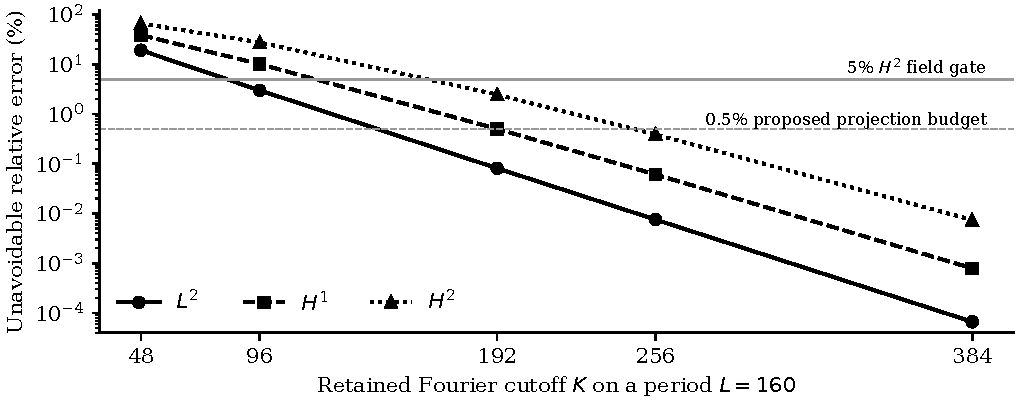
\includegraphics[width=\textwidth]{figures/projection-floor.pdf}
\caption{A lower bound on attainable errors for a strictly projected output.
The 0.5\% line is a proposed allocation of one tenth of the 5\% $H^2$ field
budget to inlet projection, not an existence criterion.}
\end{figure}
For this profile, $K=256$ is a reasonable first \emph{field-accuracy} trial under
that projection budget, with at least 513 complex Fourier coefficients and an
adequate sampling grid. A choice such as $N=1024$ represents the profile band;
full cubic residual quadrature needs more points, for example $Q_{\rm quad}=2048$.
For a trigonometric output of band $K$, the cubic RHS has band at most $3K$;
$Q_{\rm quad}>6K$ resolves its squared norm without Fourier aliasing. Audit with
a larger quadrature and finer distance sampling. This is a starting design,
not a measured memory requirement or sufficient accuracy guarantee for all profiles.

\subsection{Two additional measurement gaps}
The present solitary alignment minimizes $L^2$ distance, not $H^1$ distance.
An $H^1$ orbit diagnostic must be added and verified before reporting it.
Also, its perturbation coefficient multiplies a localized amplitude/phase
factor; it is not itself the $H^1$ norm of the perturbation. Record the actual
inlet norm or normalize directions. The generic long-distance sensitivity
implementation already uses normalized directions, but that is a separate test.

\begin{proposition}[Error in a signed neural response]\label{prop:response}
For $\delta>0$, let $w_\delta=(u_+-u_-)/(2\delta)$ and
$\widetilde w_\delta=(\widetilde u_+-\widetilde u_-)/(2\delta)$, with all four
fields in $H^1$. Then
\[
\|\widetilde w_\delta-w_\delta\|_{H^1}
\leq\frac{\|\widetilde u_+-u_+\|_{H^1}
              +\|\widetilde u_--u_-\|_{H^1}}{2\delta}.
\]
\end{proposition}
\begin{proof}
Subtract the two responses and apply the triangle inequality in $H^1$.
\end{proof}
Thus a 1\% field gate does not ensure accuracy for a perturbation of size
$10^{-3}$. Separately optimized PINNs may differ primarily because of fitting
error. Test the response against the refined numerical response directly and
report its error floor. A proposed 10\% response gate needs an absolute fallback
when the response is tiny; it is stricter information than passing the field gates.

\newpage
\section{A staged solitary-wave experiment with explicit decisions}
The following extension is \emph{proposed}, not already present in the pushed
campaign. It begins with the existing $\mu=2$, $s=0$ branch and
$\epsilon=0.025,0.05$. Broaden the branch only after the first cases qualify.
Avoid claiming novelty for solitary-wave construction or collision inelasticity
alone; both have established precedents.

\paragraph{S1. Construct and qualify the profile.}
\emph{Goal:} distinguish an actual Dysthe traveling solution from an NLS guess.
Continue from $\epsilon=0$ and evaluate the full complex traveling residual on an
oversampled grid. Refine profile grid and domain separately; recompute instead
of padding. Record residual, projection floors, spectral and boundary tails,
peak and mean flow. The local residual gate is $10^{-6}$; require refinement
agreement below the perturbation response. Failure means unresolved, not absent.
The analytic NLS control is exact on the line; its periodic-box use needs domain
checks. Refine propagation step $h/2$ separately in S2.

\paragraph{S2. Measure persistence and perturbation response.}
\emph{Goal:} distinguish shape deformation from position and phase drift.
Start with an unperturbed control and signed localized amplitude, phase and
odd-amplitude perturbations. Normalize or report their actual $H^1$ sizes.
Use sizes $10^{-3}$ and $5\times10^{-4}$, and checkpoints such as
$\Xi=1,2,4,8,20$, subject to reference/domain qualification. Save densely enough
to resolve focusing and transient growth; add samples when a peak is missed.
The evolved control measures numerical drift. The local plan saves only 21
stations through 20; increase sampling before interpreting event timing.

\paragraph{S3. Connect growth to a linearized mechanism.}
\emph{Goal:} test whether observed perturbation growth agrees with a converged
linear instability. In the moving/rotating frame the operator is real-linear:
\[
\mathcal A v=DF(Q)v+i\mu v+s\partial_\tau v.
\]
It includes variations through complex conjugation and the nonlocal mean flow.
Verify the approximate neutral directions $iQ$ and $Q'$, then refine grid and
domain and compare any positive growth rate with nonlinear propagation while
the perturbation remains small. Purely imaginary computed eigenvalues do not
prove nonlinear stability; transient growth and unresolved spectrum remain
possible. This operator is not currently implemented.

\paragraph{S4. Test a neural method on already qualified cases.}
\emph{Goal:} determine whether the selected slab PINN reproduces the numerical
wave's drift, deformation and radiation. Set the Fourier cutoff from the profile
and propagated spectral tails, rather than copying $K=48$. Retain the original
field gates, add phase/position observables, and apply a separate response gate
before making sensitivity claims. Compare a shorter slab and higher bandwidth
at matched, recorded optimization cost. Preserve every failed case and seed.

\paragraph{S5. Collisions and emergence, after S1--S4.}
\emph{Goal:} reproduce known interactions before testing learned predictions.
Compare separated Dysthe profiles with NLS at matched relative phase, separation
and speed; measure outgoing profiles and radiation with box refinement. Motion
in retarded time is not counterpropagation of physical carriers. Later, fit
generic-packet peaks to the qualified branch and check traveling residual and
lifetime. This does not establish a universal soliton-resolution conjecture.

\newpage
\section{What to measure and what counts as success}
For $v$ sampled on the periodic grid, use the consistent norms
\[
\|v\|_{H^r}^2=L\sum_m(1+k_m^2)^r|\widehat v_m|^2,
\qquad r=0,1,2.
\]
For a fixed branch profile define the proposed orbit distance
\begin{equation}\label{eq:orbit}
d_1(u,Q)=\inf_{\theta,a}
\frac{\|u-e^{i\theta}Q(\,\cdot-a\,)\|_{H^1}}{\|Q\|_{H^1}}.
\end{equation}
The branch parameters and amplitude of $Q$ stay fixed during this fit.
The symmetry-orbit viewpoint is standard in solitary-wave stability theory
\cite{gss}, but that theory's assumptions are not automatically verified here.

\begin{center}\small
\begin{tabular}{p{.25\textwidth}p{.66\textwidth}}\toprule
Observable & Interpretation and safeguard\\\midrule
Raw complex error & Tests actual prediction, retaining phase and arrival error.
Use alongside aligned error, never replace it by amplitude-only error.\\
$d_1$, fitted phase/shift & Measures deformation modulo symmetry; report phase
and position separately so a wrong speed cannot be hidden by alignment.\\
Peak, width, spectral mean & Test coherent-wave amplitude, spreading and carrier
shift. Specify how width and frequency are estimated and unwrap position.\\
Radiation measure & Report both fixed-window tail action and fitted-profile
remainder. They are diagnostic definitions, not a unique nonlinear decomposition.\\
$H^1,H^2$ and spectral tails & Check derivative growth and whether higher modes
remain resolved. Finite Fourier outputs are smooth by construction.\\
Correct invariants & Monitor action and the model's modified invariants.
Conservation alone cannot establish accuracy or a coercive regularity bound.\\
Sensitivity amplification & Normalize initial perturbations, retain signs and
check $\delta/2$. A few directions do not bound the full evolution operator.\\\bottomrule
\end{tabular}
\end{center}

Define an \emph{observed persistence distance} as the last saved station such
that all preceding saved orbit errors are below a predeclared tolerance
(for example $d_1\leq0.05$) and all numerical/domain checks pass. Report a wave
that passes at the final station as ``persists through $\Xi$''; the lifetime is
right-censored, not infinite. A 5\% threshold is an experimental choice,
not a stability theorem or a universal water-wave validity boundary.

Numerical evidence for a loss of regularity would require growth that survives
independent grid/step/domain refinement and increasing spectral bandwidth.
A rising tail at the cutoff usually first establishes under-resolution.
Distinguish that from optimization failure, boundary return and physical-model
breakdown. Failure to observe growth likewise does not prove global smoothness.

\newpage
\section{How PINNs and FNOs should be used here}
\subsection{Slab PINN: a separately fitted solution on successive intervals}
A slab PINN solves $[\xi_j,\xi_{j+1}]$, passes its predicted endpoint to the next
slab, and repeats. The current implementation uses a network in $\xi$ that
outputs complex Fourier coefficients in $\tau$; this enforces periodicity and
permits complete-slice evaluation of $\absD(|u|^2)$. It does not sample the
nonlocal term from disconnected points. Numerical labels are reserved for
auditing; slab endpoints must not be reset to the reference during evaluation.

Sequence training has methodological support in PINN failure-mode work
\cite{failure}. Wang et al.'s causal weighting is a related but distinct
algorithm \cite{causal}: sequential slabs alone are not their specific residual
weighting rule. Any added weighting should be a separately tested ablation.
Residual minimization measures equation fit over the fitted interval, not
forecast generalization or an existence certificate.

For solitary waves, first compare the existing spectral correction against a
known moving/rotating reference representation, both with the same inlet and
full residual. A moving frame may reduce phase/translation learning burden,
but it must not freeze amplitude or suppress admissible perturbations. The
benefit is a hypothesis to measure, not an established Dysthe result.

\subsection{FNO: learn across initial functions, not one profile}
FNO learns an operator from a family of functions \cite{fno}; duplicating one
profile with many snapshots does not provide many independent inlets. A useful
new dataset would span qualified branch parameters, global phase, translations,
and controlled amplitude/phase/radiative perturbations, then include generic
packet controls. Keep all snapshots, augmentations, signed perturbations and
refinements of a parent inlet in one train/validation/test group.

Compare the same architecture trained with data loss against a PINO residual
augmentation \cite{pino}, using equal data, seeds and recorded cost. Freeze the
choice on validation fields before test inspection. Evaluate short-step accuracy
and autonomous rollout without reference resets. Separate interpolation within
the sampled branch from held-out amplitude/steepness ranges. More epochs alone
are not a supported remedy for the existing pilot failures.

An ordinary FNO's latent Fourier cutoff does not by itself strictly limit its
output, because local nonlinear layers can create higher frequencies. The
projection floor in Section~\ref{sec:projection} applies to the explicit output projector used in
this project's spectral models. Record latent modes, output cutoff and grid
separately. Phase/translation augmentation tests physical symmetries but should
not inflate the independent test count.

\subsection{Priority and cost}
Run reference qualification and the slab PINN extension first. Treat FNO recovery
as a separate controlled operator study. On A100, record data generation,
optimization, validation, checkpoint I/O, evaluation and peak memory; compare
total cost at matched measured accuracy against the Fourier solver. A cached
neural forward pass is not the cost of obtaining a new per-inlet PINN solution.

\newpage
\section{Recommended research claim and verification record}
The near-term question is:
\begin{quote}
For a specified family of resolved spatial free-surface Dysthe solitary waves,
how do perturbation growth, phase/position drift and radiation depend on
steepness and propagation distance, and which of these behaviors can a slab
PINN or an operator model reproduce within a measured error budget?
\end{quote}
This can produce useful numerical evidence without promising a global existence
proof. A subsequent proof project could study small-$\epsilon$ continuation
from NLS or validated a-posteriori existence, but would need explicit function
spaces, kernel removal, nonlocal estimates and validated inverse/tail bounds.
Neither a converged iteration nor an ML residual supplies these ingredients.

\paragraph{Immediate changes justified by this review.}
Make the solitary workflow self-contained; add $H^1$ orbit fitting and normalized
perturbation reporting; select bandwidth from projection/refinement evidence;
increase event sampling; and keep response accuracy separate from field accuracy.
The real-linear spectral operator is a later explicit implementation task.
The report does not claim these proposed changes have been implemented or pushed.

\paragraph{Evidence inspected.}
The audit checked remote branch identities, the CPU-only CI record, published
configs/results, local solitary source and the stored smoke checksum. Scientific
CPU science trajectories were not rerun. New calculations covered Fourier
projection and aggregate consistency. The exact published source passed all 39
software tests, including bounded training/restart checks, plus scope and artifact
validation; see \texttt{data/remote-audit.json}. The new results commit changes
no source. Its metadata were downloaded and hash-checked. No HPC job was
submitted by this review and no cluster filesystem inspected. Detailed
qualification, raw trajectories and failure logs are reported at the manifest's
source location. NLS methodology is not relabeled as Dysthe validation.

\paragraph{Reproducible report package.}
\texttt{review.tex}, \texttt{royden-report.sty}, the three vector PDF figures,
\texttt{make\_figures.py}, and archived data are self-contained. Spectral powers
reproduce \eqref{eq:floor}; the JSON records the source NPZ checksum.
\texttt{verification.json} records pdfLaTeX compilation and rendered-page checks.
Preprint assumptions were inspected; proofs were not independently formalized.

\paragraph{Reviewed source identities.}
\begin{itemize}
\item Experiment source: \texttt{c04b44ba6459cac6f216e3a59de4fac78e3b55d7}.
\item Results publication: \texttt{723883f27a6b3489bfc36f55d9d15b52e8635ad0}.
\item Core dependency: \texttt{a47a42321475feb6bc55031f4b752419f4b7fda9}.
\item Learning dependency: \texttt{db7274f8cfe959cf187351f56b3dd4bf89f0e9b4}.
\end{itemize}
Historical solitary evidence remains distinct from those published commits.
Its source NPZ has SHA256
\begin{center}\footnotesize
\texttt{63e8636ed53c3183c6f5c2abb246ed4e62d0a97499c0f7029f104de198e21123}.
\end{center}

\clearpage
\begin{thebibliography}{99}\small
\bibitem{fd} F. Fedele and D. Dutykh, \emph{Hamiltonian description and traveling
waves of the spatial Dysthe equations}, preprint 2011, version 3, 12 April 2012.
\url{https://arxiv.org/abs/1110.3605v3}.
\bibitem{akylas} T. R. Akylas, \emph{Higher-order modulation effects on solitary
wave envelopes in deep water}, Journal of Fluid Mechanics 198 (1989), 387--397.
\url{https://doi.org/10.1017/S0022112089000182}.
\bibitem{ekk} A. Esfahani, A. Kairzhan and M. Karazym, \emph{Traveling waves for
nonlocal derivative nonlinear Schr\"odinger equations: a variational
characterization}, preprint, version 4, 21 September 2026.
\url{https://arxiv.org/abs/2603.22482v4}.
\bibitem{sy} A. J. Sutherland and S. C. Yim, \emph{Six-wave scattering in
Hamiltonian Dysthe equations: Euler matching and integrability obstructions},
preprint, version 1, 19 September 2026.
\url{https://arxiv.org/abs/2609.23175v1}.
\bibitem{si2025} C. M. Schober and A. Islas, \emph{Soliton-like rogue wave
dynamics in dissipative higher-order nonlinear Schr\"odinger models: a Floquet
spectral perspective}, Studies in Applied Mathematics 155(6) (2025), e70150.
Publisher abstract inspected. \url{https://doi.org/10.1111/sapm.70150}.
\bibitem{tikan} A. Tikan et al., \emph{Nonlinear dispersion relation in integrable
turbulence}, Scientific Reports 12 (2022), 10386.
\url{https://doi.org/10.1038/s41598-022-14209-7}.
\bibitem{si2026} C. M. Schober and A. Islas, \emph{Higher-order extensions of
weakly viscous Dysthe theory and a phase-lag model for nonlinear mean-flow
damping}, preprint, version 1, 5 August 2026.
\url{https://arxiv.org/abs/2608.04473v1}.
\bibitem{mps} R. Mosincat, D. Pilod and J.-C. Saut, \emph{Global well-posedness
and scattering for the Dysthe equation in $L^2(\mathbb R^2)$}, preprint (2020).
\url{https://arxiv.org/abs/2007.01613}.
\bibitem{gss} M. Grillakis, J. Shatah and W. Strauss, \emph{Stability theory of
solitary waves in the presence of symmetry, I}, Journal of Functional Analysis
74 (1987), 160--197. \url{https://doi.org/10.1016/0022-1236(87)90044-9}.
\bibitem{failure} A. S. Krishnapriyan et al., \emph{Characterizing possible failure
modes in physics-informed neural networks}, NeurIPS 34 (2021), 26548--26560.
\url{https://arxiv.org/abs/2109.01050}.
\bibitem{causal} S. Wang, S. Sankaran and P. Perdikaris, \emph{Respecting causality
for training physics-informed neural networks}, Computer Methods in Applied
Mechanics and Engineering 421 (2024), 116813.
\url{https://doi.org/10.1016/j.cma.2024.116813}.
\bibitem{fno} Z. Li et al., \emph{Fourier neural operator for parametric partial
differential equations}, ICLR (2021); preprint first posted 2020.
\url{https://arxiv.org/abs/2010.08895}.
\bibitem{pino} Z. Li et al., \emph{Physics-informed neural operator for learning
partial differential equations}, ACM/IMS Journal of Data Science (2024);
preprint first posted 2021. \url{https://doi.org/10.1145/3648506}.
\end{thebibliography}
\end{document}
